
% Copyright (c) 2015 - 2019 Mario Mlačak, mmlacak@gmail.com
% Licensed and published as Public Domain work.

% Nineteen chapter ====================================================
\chapter*{Nineteen}
\addcontentsline{toc}{chapter}{Nineteen}

\begin{flushright}
\parbox{0.8\textwidth}{
\emph{The truth is at the beginning of anything and its end are alike touching. \\
\hspace*{\fill}{\textperiodcentered \textperiodcentered \textperiodcentered \hspace*{0.2em} Yoshida Kenko} } }
\end{flushright}

\noindent
Nineteen is chess variant which is played on 18 x 18 board, with
light gold-yellow and white fields and gold-yellow and dark gray
pieces. In algebraic notation, columns are enumerated from 'a' to 'r',
and rows are enumerated from '1' to '18'. A new piece is introduced,
Star.

\clearpage % ..........................................................
% Star ****************************************************************

\section*{Star}
\addcontentsline{toc}{section}{Star}

% \vspace*{-1.3\baselineskip}
\noindent
\begin{wrapfigure}[11]{l}{0.4\textwidth}
\centering
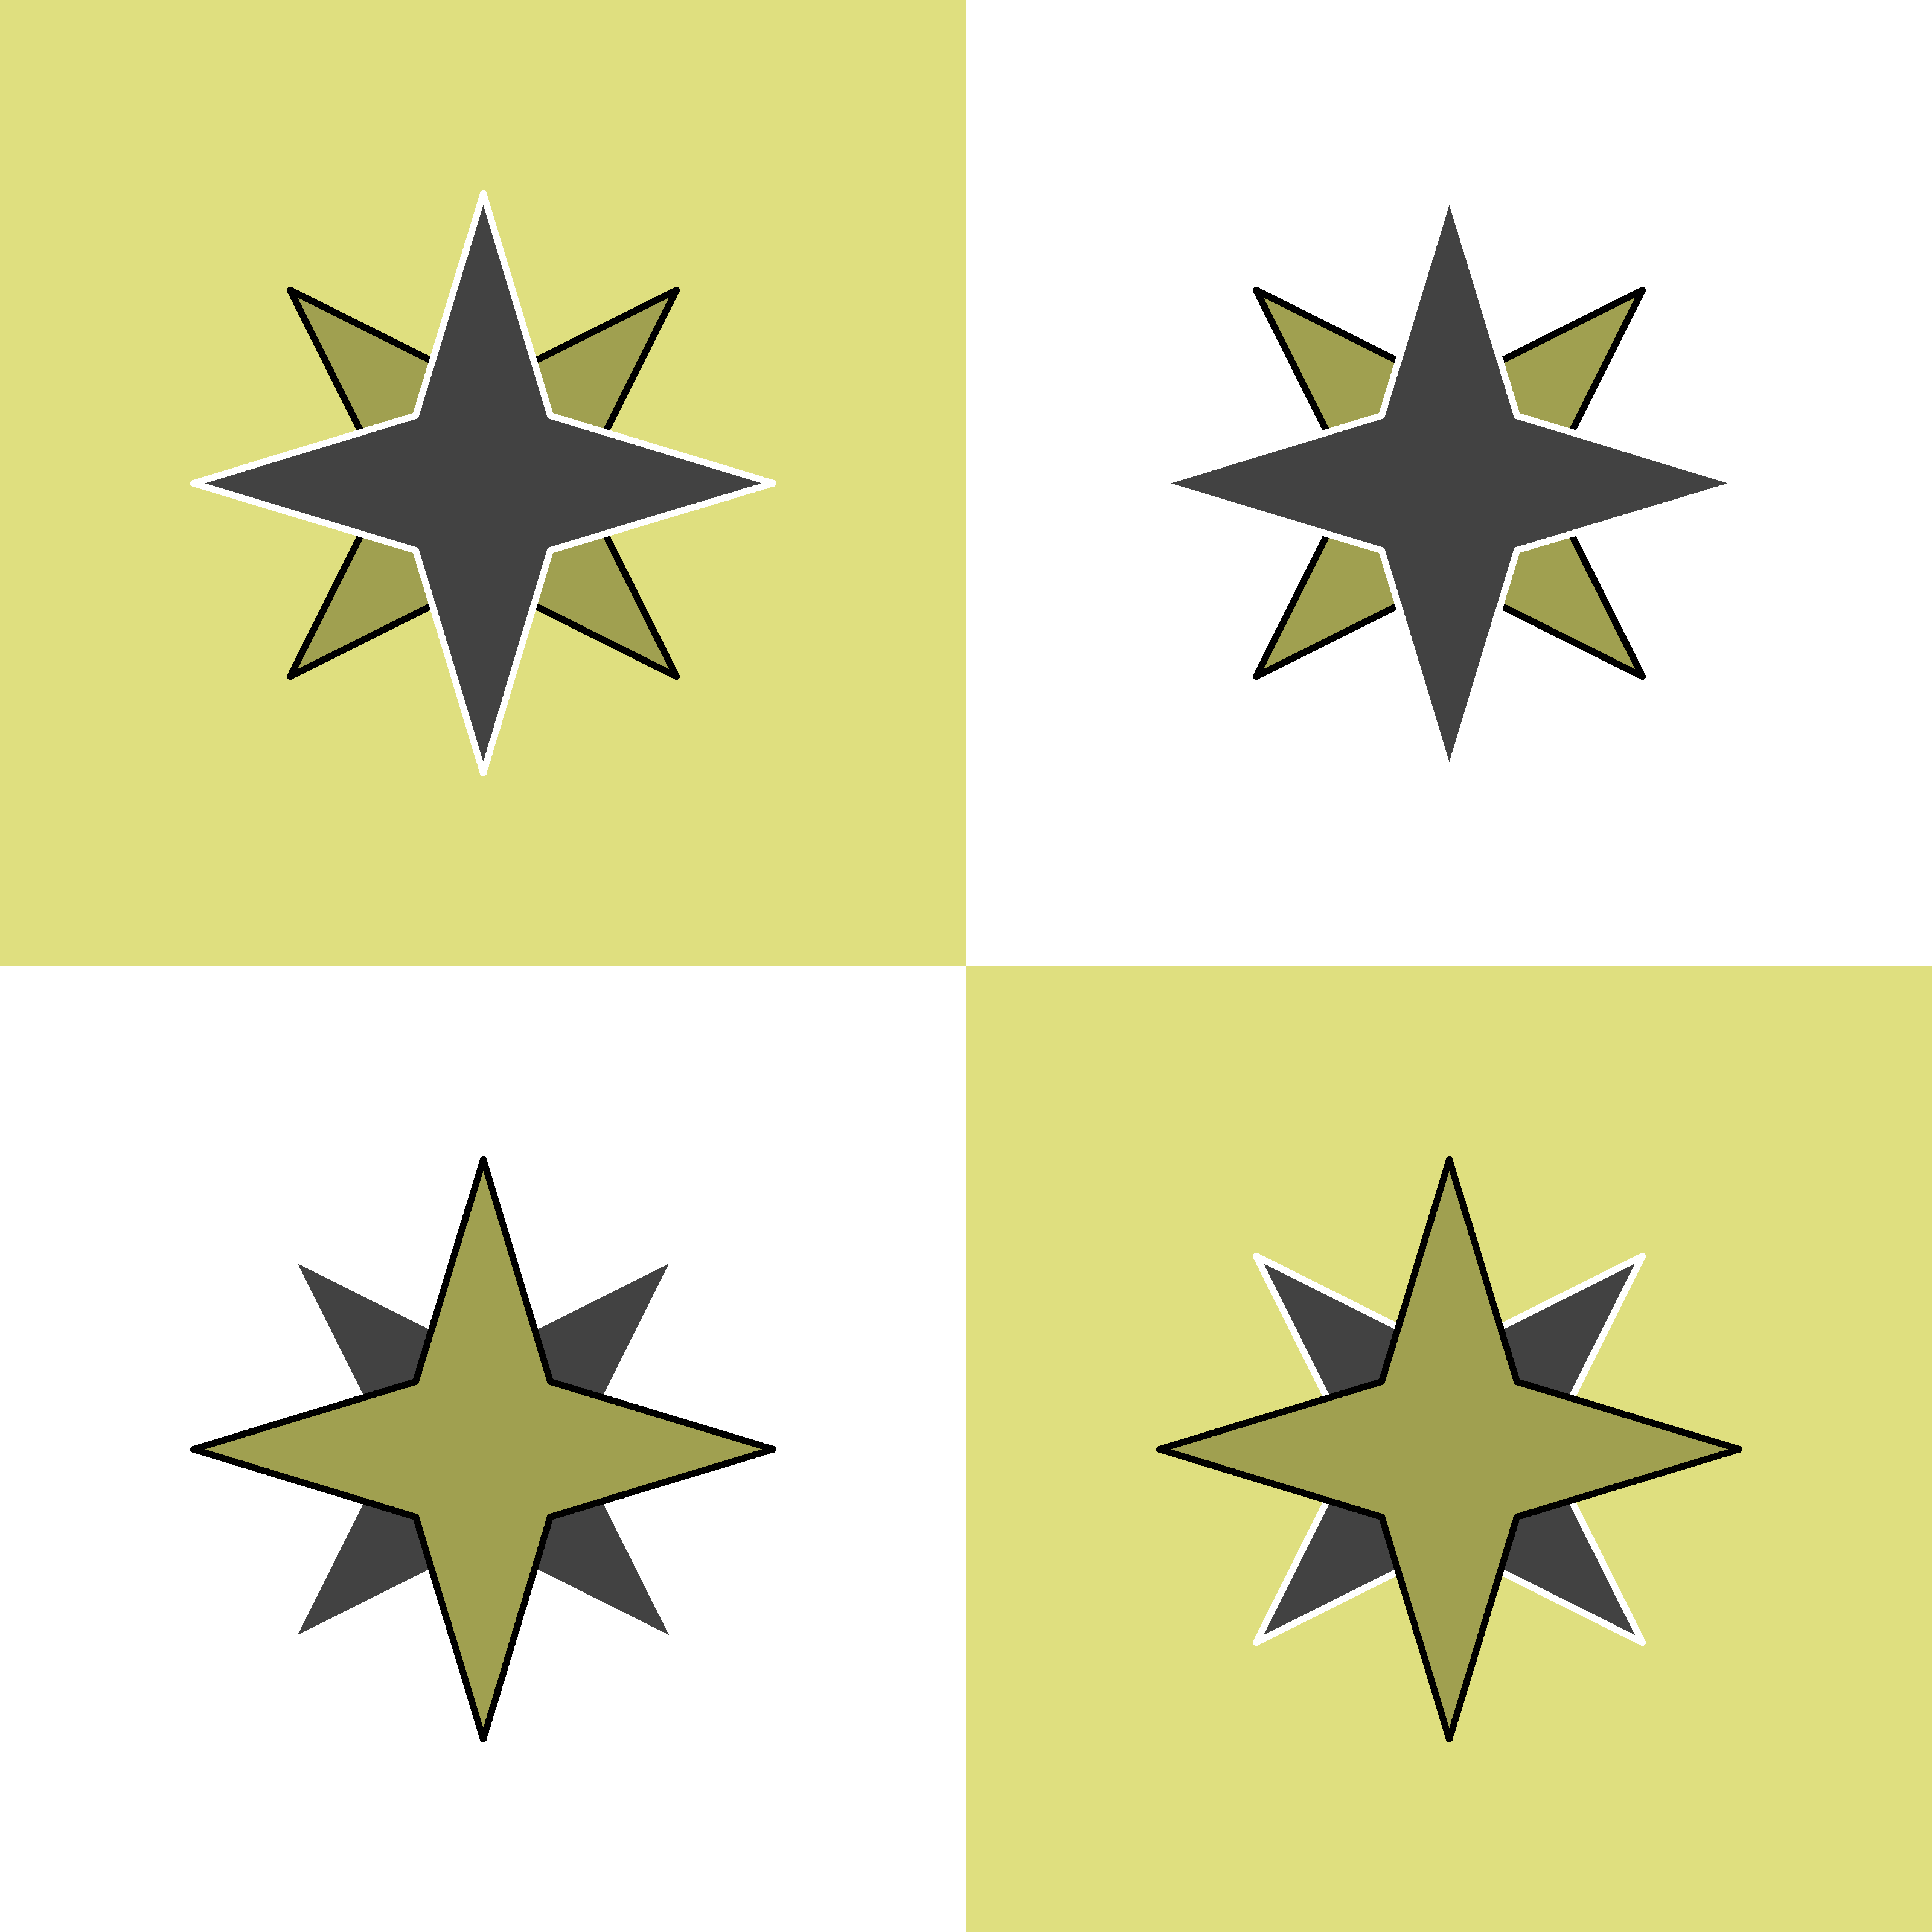
\includegraphics[width=0.4\textwidth, keepaspectratio=true]{pieces/11_star.png}
\caption{Star}
\label{fig:11_star}
\end{wrapfigure}
Star does not belong to any player, and can't be moved, activated, captured or converted by
either. Light Stars are positioned in lower left and upper right corners, dark Stars in lower
right and upper left corners.

Star is a teleporting piece. Teleportation is initiated by touching a Star or field at which
it stands with a piece (as if trying to capture a Star). Piece in question, if it's not Wave,
then reappears on any empty portal-field near Star in opposite color. Any momentum carried is
lost. Teleportation is not limited by matching colors of a piece and a Star, any piece can use
any Star to start teleporting.

Player initiating teleportation can choose which opposite color Star will be destination,
and at which empty portal-field piece will reappear. If there is no empty portal-field near
both Stars of opposite color, piece is removed from chessboard as if it has been captured.

If teleported piece is Wave, it continues movement as if activated on a field occupied by
other Star in the same color. Wave retains all of momentum carried into teleportation.
The way and direction of movement of Wave is the same as before teleportation.

Kings cannot be teleported.
Pawns cannot be promoted to a Star.
In algebraic notation symbol for Star is 'T'.

\clearpage % ..........................................................

\subsection*{Portal-fields}
\addcontentsline{toc}{subsection}{Portal-fields}

\noindent
\begin{figure}[!h]
% \begin{figure}[!t]
\includegraphics[width=1.0\textwidth, keepaspectratio=true]{examples/12_n/scn_n_01_portal_fields.png}
\caption{Portal-fields}
\label{fig:scn_n_01_portal_fields}
% \centering
\end{figure}

Portal-fields are all fields immediately surrounding a particular field
horizontally, vertically and diagonally. They are the same as step-fields
of a King.

Since all Stars are pinned into the corners of a chessboard, there are always
exactly 3 portal-fields around each one.

\clearpage % ..........................................................

\subsection*{Teleporting pieces}
\addcontentsline{toc}{subsection}{Teleporting pieces}

\noindent
\begin{figure}[!h]
% \begin{figure}[!t]
\includegraphics[width=1.0\textwidth, keepaspectratio=true]{examples/12_n/scn_n_02_teleport_init.png}
\caption{Teleportation start}
\label{fig:scn_n_02_teleport_init}
% \centering
\end{figure}

...

\clearpage % ..........................................................

\noindent
\begin{figure}[!h]
% \begin{figure}[!t]
\includegraphics[width=1.0\textwidth, keepaspectratio=true]{examples/12_n/scn_n_03_teleport_move_2.png}
\caption{Teleporting dark}
\label{fig:scn_n_03_teleport_move_2}
% \centering
\end{figure}

...

\clearpage % ..........................................................

\noindent
\begin{figure}[!h]
% \begin{figure}[!t]
\includegraphics[width=1.0\textwidth, keepaspectratio=true]{examples/12_n/scn_n_04_teleport_move_3.png}
\caption{Teleporting light}
\label{fig:scn_n_04_teleport_move_3}
% \centering
\end{figure}

...

\clearpage % ..........................................................

\noindent
\begin{figure}[!h]
% \begin{figure}[!t]
\includegraphics[width=1.0\textwidth, keepaspectratio=true]{examples/12_n/scn_n_05_teleport_end.png}
\caption{Teleportation end}
\label{fig:scn_n_05_teleport_end}
% \centering
\end{figure}

...

% \label{fig:scn_mv_18_activating_rush_pawn_init}

\clearpage % ..........................................................

\subsubsection*{Teleporting Wave}
\addcontentsline{toc}{subsubsection}{Teleporting Wave}

\huge{TODO}
\normalsize{}

Teleporting Wave ... does preserve momentum, others do not.

Activating Wave ...

Activated \& teleported Wave ... by Unicorn on board edge ... continuity of alterations between step directions

\clearpage % ..........................................................

\subsubsection*{Teleporting Bishop}
\addcontentsline{toc}{subsubsection}{Teleporting Bishop}

\huge{TODO}
\normalsize{}

Teleporting Bishop ... changing color of accessible fields.

\clearpage % ..........................................................

\subsubsection*{Teleporting Pawn}
\addcontentsline{toc}{subsubsection}{Teleporting Pawn}

\huge{TODO}
\normalsize{}

Teleporting Pawn ... from step-fields, capture-fields ... promotion \& tagging for it.

% **************************************************************** Star
\clearpage % ..........................................................

\section*{Promotion}
\addcontentsline{toc}{section}{Promotion}

Promotion is non enforced, delayed variety, i.e. it's the same as in
\hyperref[sec:Age of Aquarius/Promotion]{previous chess variant}, Age of Aquarius.

Again, Pawns cannot be promoted to a Star.

Additionaly, promotion in this variant is monogamous.
Only one Queen in the same color can be present on chessboard at any given time.

\clearpage % ..........................................................

\section*{En passant}
\addcontentsline{toc}{section}{En passant}

\noindent
\begin{wrapfigure}{l}{0.4\textwidth}
\centering
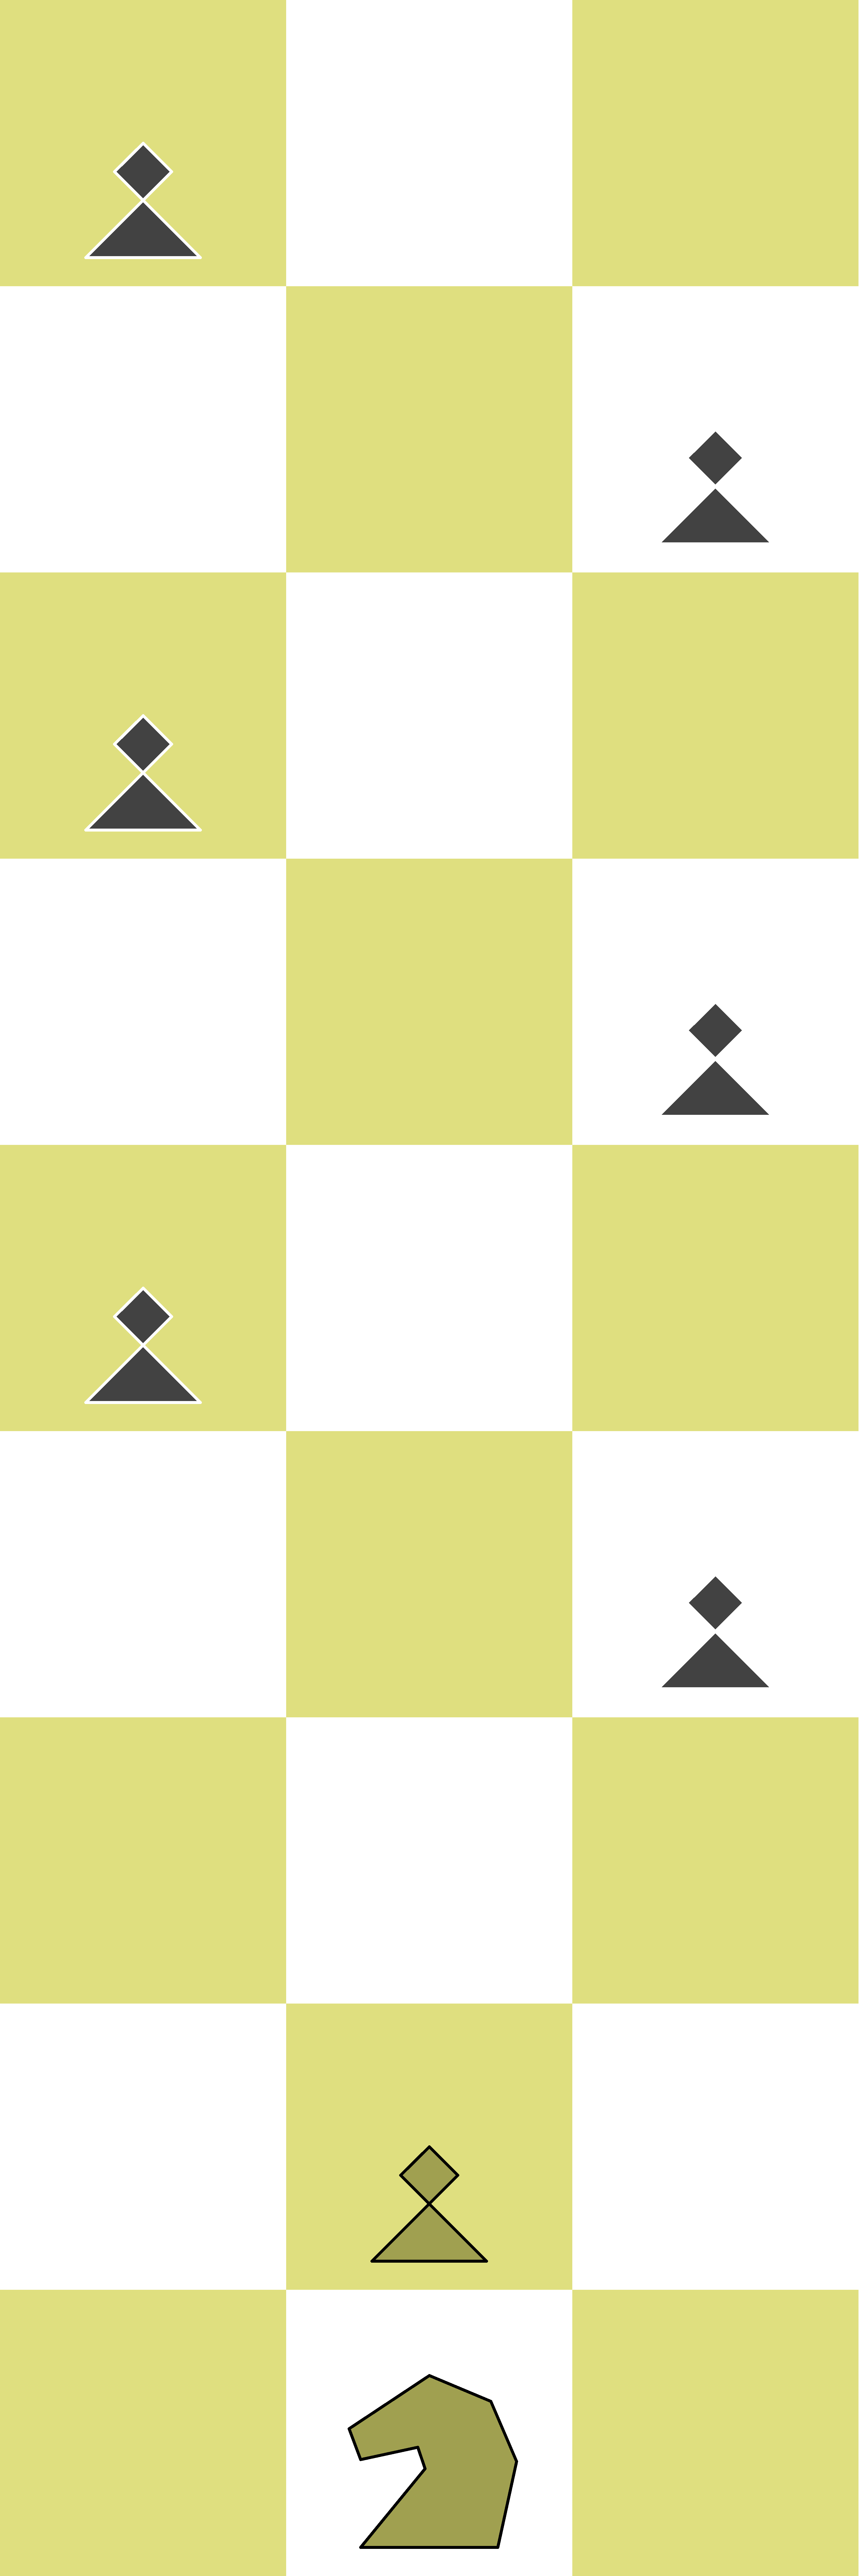
\includegraphics[width=0.166666666667\textwidth, keepaspectratio=true]{en_passants/12_nineteen_en_passant.png}
\caption{En passant}
\label{fig:12_nineteen_en_passant}
\end{wrapfigure}
Rush and en passant are identical to those in Classic Chess, only difference
is that Pawn can now move longer on initial turn, up to 7 fields in this
variant.

\clearpage % ..........................................................

\section*{Castling}
\addcontentsline{toc}{section}{Castling}

Castling is the same as in Classical Chess, only difference is that King can move between 2 and 6 fields across.
All other constraints from Classical Chess still applies.

\noindent
\begin{figure}[!h]
% \begin{figure}[!t]
\includegraphics[width=1.0\textwidth, keepaspectratio=true]{castlings/12_n/nineteen_castling.png}
\caption{Castling}
\label{fig:nineteen_castling}
% \centering
\end{figure}

In example above, all valid King's castling moves are numbered.

\noindent
\begin{figure}[!h]
% \begin{figure}[!t]
\includegraphics[width=1.0\textwidth, keepaspectratio=true]{castlings/12_n/nineteen_castling_left_05.png}
\caption{Castling long left}
\label{fig:nineteen_castling_left_05}
% \centering
\end{figure}

In this example King was castling long to the left. Initial King's position is marked with "K".
After castling is finished, left Rook ends up at field immediately right to the King.

\clearpage % ..........................................................

\section*{Initial setup}
\addcontentsline{toc}{section}{Initial setup}

Stars are positioned in very corners of chessboard, light Stars in lower left and upper right
corners, dark Stars in lower right and upper left corners. Initial setup can be seen in image below:

\noindent
% \begin{figure}[t]
\begin{figure}[h]
\includegraphics[width=1.0\textwidth, keepaspectratio=true]{boards/12_nineteen.png}
\caption{Nineteen board}
\label{fig:12_nineteen}
% \centering
\end{figure}

\clearpage % ..........................................................
% ==================================================== Nineteen chapter
